% Created by tikzDevice version 0.12.3.1 on 2022-02-28 16:49:15
% !TEX encoding = UTF-8 Unicode
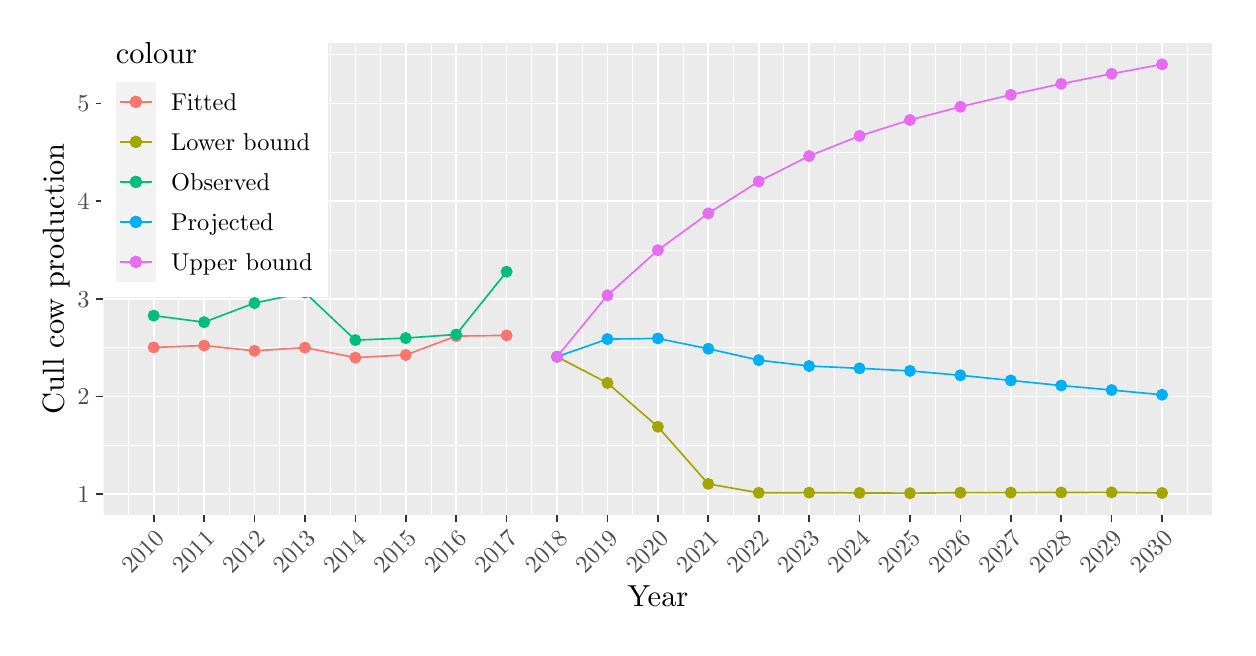
\begin{tikzpicture}[x=1pt,y=1pt]
\definecolor{fillColor}{RGB}{255,255,255}
\path[use as bounding box,fill=fillColor,fill opacity=0.00] (0,0) rectangle (433.62,216.81);
\begin{scope}
\path[clip] (  0.00,  0.00) rectangle (433.62,216.81);
\definecolor{drawColor}{RGB}{255,255,255}
\definecolor{fillColor}{RGB}{255,255,255}

\path[draw=drawColor,line width= 0.6pt,line join=round,line cap=round,fill=fillColor] (  0.00,  0.00) rectangle (433.62,216.81);
\end{scope}
\begin{scope}
\path[clip] ( 27.31, 40.85) rectangle (428.12,211.31);
\definecolor{fillColor}{gray}{0.92}

\path[fill=fillColor] ( 27.31, 40.85) rectangle (428.12,211.31);
\definecolor{drawColor}{RGB}{255,255,255}

\path[draw=drawColor,line width= 0.3pt,line join=round] ( 27.31, 65.87) --
	(428.12, 65.87);

\path[draw=drawColor,line width= 0.3pt,line join=round] ( 27.31,101.18) --
	(428.12,101.18);

\path[draw=drawColor,line width= 0.3pt,line join=round] ( 27.31,136.50) --
	(428.12,136.50);

\path[draw=drawColor,line width= 0.3pt,line join=round] ( 27.31,171.81) --
	(428.12,171.81);

\path[draw=drawColor,line width= 0.3pt,line join=round] ( 27.31,207.12) --
	(428.12,207.12);

\path[draw=drawColor,line width= 0.3pt,line join=round] ( 27.31, 40.85) --
	( 27.31,211.31);

\path[draw=drawColor,line width= 0.3pt,line join=round] ( 36.42, 40.85) --
	( 36.42,211.31);

\path[draw=drawColor,line width= 0.3pt,line join=round] ( 54.64, 40.85) --
	( 54.64,211.31);

\path[draw=drawColor,line width= 0.3pt,line join=round] ( 72.86, 40.85) --
	( 72.86,211.31);

\path[draw=drawColor,line width= 0.3pt,line join=round] ( 91.08, 40.85) --
	( 91.08,211.31);

\path[draw=drawColor,line width= 0.3pt,line join=round] (109.30, 40.85) --
	(109.30,211.31);

\path[draw=drawColor,line width= 0.3pt,line join=round] (127.51, 40.85) --
	(127.51,211.31);

\path[draw=drawColor,line width= 0.3pt,line join=round] (145.73, 40.85) --
	(145.73,211.31);

\path[draw=drawColor,line width= 0.3pt,line join=round] (163.95, 40.85) --
	(163.95,211.31);

\path[draw=drawColor,line width= 0.3pt,line join=round] (182.17, 40.85) --
	(182.17,211.31);

\path[draw=drawColor,line width= 0.3pt,line join=round] (200.39, 40.85) --
	(200.39,211.31);

\path[draw=drawColor,line width= 0.3pt,line join=round] (218.61, 40.85) --
	(218.61,211.31);

\path[draw=drawColor,line width= 0.3pt,line join=round] (236.83, 40.85) --
	(236.83,211.31);

\path[draw=drawColor,line width= 0.3pt,line join=round] (255.04, 40.85) --
	(255.04,211.31);

\path[draw=drawColor,line width= 0.3pt,line join=round] (273.26, 40.85) --
	(273.26,211.31);

\path[draw=drawColor,line width= 0.3pt,line join=round] (291.48, 40.85) --
	(291.48,211.31);

\path[draw=drawColor,line width= 0.3pt,line join=round] (309.70, 40.85) --
	(309.70,211.31);

\path[draw=drawColor,line width= 0.3pt,line join=round] (327.92, 40.85) --
	(327.92,211.31);

\path[draw=drawColor,line width= 0.3pt,line join=round] (346.14, 40.85) --
	(346.14,211.31);

\path[draw=drawColor,line width= 0.3pt,line join=round] (364.36, 40.85) --
	(364.36,211.31);

\path[draw=drawColor,line width= 0.3pt,line join=round] (382.57, 40.85) --
	(382.57,211.31);

\path[draw=drawColor,line width= 0.3pt,line join=round] (400.79, 40.85) --
	(400.79,211.31);

\path[draw=drawColor,line width= 0.3pt,line join=round] (419.01, 40.85) --
	(419.01,211.31);

\path[draw=drawColor,line width= 0.3pt,line join=round] (428.12, 40.85) --
	(428.12,211.31);

\path[draw=drawColor,line width= 0.6pt,line join=round] ( 27.31, 48.22) --
	(428.12, 48.22);

\path[draw=drawColor,line width= 0.6pt,line join=round] ( 27.31, 83.53) --
	(428.12, 83.53);

\path[draw=drawColor,line width= 0.6pt,line join=round] ( 27.31,118.84) --
	(428.12,118.84);

\path[draw=drawColor,line width= 0.6pt,line join=round] ( 27.31,154.15) --
	(428.12,154.15);

\path[draw=drawColor,line width= 0.6pt,line join=round] ( 27.31,189.46) --
	(428.12,189.46);

\path[draw=drawColor,line width= 0.6pt,line join=round] ( 45.53, 40.85) --
	( 45.53,211.31);

\path[draw=drawColor,line width= 0.6pt,line join=round] ( 63.75, 40.85) --
	( 63.75,211.31);

\path[draw=drawColor,line width= 0.6pt,line join=round] ( 81.97, 40.85) --
	( 81.97,211.31);

\path[draw=drawColor,line width= 0.6pt,line join=round] (100.19, 40.85) --
	(100.19,211.31);

\path[draw=drawColor,line width= 0.6pt,line join=round] (118.41, 40.85) --
	(118.41,211.31);

\path[draw=drawColor,line width= 0.6pt,line join=round] (136.62, 40.85) --
	(136.62,211.31);

\path[draw=drawColor,line width= 0.6pt,line join=round] (154.84, 40.85) --
	(154.84,211.31);

\path[draw=drawColor,line width= 0.6pt,line join=round] (173.06, 40.85) --
	(173.06,211.31);

\path[draw=drawColor,line width= 0.6pt,line join=round] (191.28, 40.85) --
	(191.28,211.31);

\path[draw=drawColor,line width= 0.6pt,line join=round] (209.50, 40.85) --
	(209.50,211.31);

\path[draw=drawColor,line width= 0.6pt,line join=round] (227.72, 40.85) --
	(227.72,211.31);

\path[draw=drawColor,line width= 0.6pt,line join=round] (245.94, 40.85) --
	(245.94,211.31);

\path[draw=drawColor,line width= 0.6pt,line join=round] (264.15, 40.85) --
	(264.15,211.31);

\path[draw=drawColor,line width= 0.6pt,line join=round] (282.37, 40.85) --
	(282.37,211.31);

\path[draw=drawColor,line width= 0.6pt,line join=round] (300.59, 40.85) --
	(300.59,211.31);

\path[draw=drawColor,line width= 0.6pt,line join=round] (318.81, 40.85) --
	(318.81,211.31);

\path[draw=drawColor,line width= 0.6pt,line join=round] (337.03, 40.85) --
	(337.03,211.31);

\path[draw=drawColor,line width= 0.6pt,line join=round] (355.25, 40.85) --
	(355.25,211.31);

\path[draw=drawColor,line width= 0.6pt,line join=round] (373.46, 40.85) --
	(373.46,211.31);

\path[draw=drawColor,line width= 0.6pt,line join=round] (391.68, 40.85) --
	(391.68,211.31);

\path[draw=drawColor,line width= 0.6pt,line join=round] (409.90, 40.85) --
	(409.90,211.31);
\definecolor{drawColor}{RGB}{248,118,109}

\path[draw=drawColor,line width= 0.6pt,line join=round] ( 45.53,101.27) --
	( 63.75,101.94) --
	( 81.97,100.03) --
	(100.19,101.20) --
	(118.41, 97.58) --
	(136.62, 98.55) --
	(154.84,105.36) --
	(173.06,105.62);
\definecolor{fillColor}{RGB}{248,118,109}

\path[draw=drawColor,line width= 0.4pt,line join=round,line cap=round,fill=fillColor] ( 45.53,101.27) circle (  1.96);

\path[draw=drawColor,line width= 0.4pt,line join=round,line cap=round,fill=fillColor] ( 63.75,101.94) circle (  1.96);

\path[draw=drawColor,line width= 0.4pt,line join=round,line cap=round,fill=fillColor] ( 81.97,100.03) circle (  1.96);

\path[draw=drawColor,line width= 0.4pt,line join=round,line cap=round,fill=fillColor] (100.19,101.20) circle (  1.96);

\path[draw=drawColor,line width= 0.4pt,line join=round,line cap=round,fill=fillColor] (118.41, 97.58) circle (  1.96);

\path[draw=drawColor,line width= 0.4pt,line join=round,line cap=round,fill=fillColor] (136.62, 98.55) circle (  1.96);

\path[draw=drawColor,line width= 0.4pt,line join=round,line cap=round,fill=fillColor] (154.84,105.36) circle (  1.96);

\path[draw=drawColor,line width= 0.4pt,line join=round,line cap=round,fill=fillColor] (173.06,105.62) circle (  1.96);
\definecolor{drawColor}{RGB}{0,191,125}

\path[draw=drawColor,line width= 0.6pt,line join=round] ( 45.53,112.76) --
	( 63.75,110.39) --
	( 81.97,117.31) --
	(100.19,121.09) --
	(118.41,103.91) --
	(136.62,104.65) --
	(154.84,105.94) --
	(173.06,128.64);
\definecolor{fillColor}{RGB}{0,191,125}

\path[draw=drawColor,line width= 0.4pt,line join=round,line cap=round,fill=fillColor] ( 45.53,112.76) circle (  1.96);

\path[draw=drawColor,line width= 0.4pt,line join=round,line cap=round,fill=fillColor] ( 63.75,110.39) circle (  1.96);

\path[draw=drawColor,line width= 0.4pt,line join=round,line cap=round,fill=fillColor] ( 81.97,117.31) circle (  1.96);

\path[draw=drawColor,line width= 0.4pt,line join=round,line cap=round,fill=fillColor] (100.19,121.09) circle (  1.96);

\path[draw=drawColor,line width= 0.4pt,line join=round,line cap=round,fill=fillColor] (118.41,103.91) circle (  1.96);

\path[draw=drawColor,line width= 0.4pt,line join=round,line cap=round,fill=fillColor] (136.62,104.65) circle (  1.96);

\path[draw=drawColor,line width= 0.4pt,line join=round,line cap=round,fill=fillColor] (154.84,105.94) circle (  1.96);

\path[draw=drawColor,line width= 0.4pt,line join=round,line cap=round,fill=fillColor] (173.06,128.64) circle (  1.96);
\definecolor{drawColor}{RGB}{163,165,0}

\path[draw=drawColor,line width= 0.6pt,line join=round] (191.28, 97.91) --
	(209.50, 88.42) --
	(227.72, 72.60) --
	(245.94, 51.95) --
	(264.15, 48.74) --
	(282.37, 48.79) --
	(300.59, 48.70) --
	(318.81, 48.60) --
	(337.03, 48.78) --
	(355.25, 48.80) --
	(373.46, 48.84) --
	(391.68, 48.90) --
	(409.90, 48.66);
\definecolor{fillColor}{RGB}{163,165,0}

\path[draw=drawColor,line width= 0.4pt,line join=round,line cap=round,fill=fillColor] (191.28, 97.91) circle (  1.96);

\path[draw=drawColor,line width= 0.4pt,line join=round,line cap=round,fill=fillColor] (209.50, 88.42) circle (  1.96);

\path[draw=drawColor,line width= 0.4pt,line join=round,line cap=round,fill=fillColor] (227.72, 72.60) circle (  1.96);

\path[draw=drawColor,line width= 0.4pt,line join=round,line cap=round,fill=fillColor] (245.94, 51.95) circle (  1.96);

\path[draw=drawColor,line width= 0.4pt,line join=round,line cap=round,fill=fillColor] (264.15, 48.74) circle (  1.96);

\path[draw=drawColor,line width= 0.4pt,line join=round,line cap=round,fill=fillColor] (282.37, 48.79) circle (  1.96);

\path[draw=drawColor,line width= 0.4pt,line join=round,line cap=round,fill=fillColor] (300.59, 48.70) circle (  1.96);

\path[draw=drawColor,line width= 0.4pt,line join=round,line cap=round,fill=fillColor] (318.81, 48.60) circle (  1.96);

\path[draw=drawColor,line width= 0.4pt,line join=round,line cap=round,fill=fillColor] (337.03, 48.78) circle (  1.96);

\path[draw=drawColor,line width= 0.4pt,line join=round,line cap=round,fill=fillColor] (355.25, 48.80) circle (  1.96);

\path[draw=drawColor,line width= 0.4pt,line join=round,line cap=round,fill=fillColor] (373.46, 48.84) circle (  1.96);

\path[draw=drawColor,line width= 0.4pt,line join=round,line cap=round,fill=fillColor] (391.68, 48.90) circle (  1.96);

\path[draw=drawColor,line width= 0.4pt,line join=round,line cap=round,fill=fillColor] (409.90, 48.66) circle (  1.96);
\definecolor{drawColor}{RGB}{0,176,246}

\path[draw=drawColor,line width= 0.6pt,line join=round] (191.28, 97.91) --
	(209.50,104.28) --
	(227.72,104.51) --
	(245.94,100.79) --
	(264.15, 96.67) --
	(282.37, 94.55) --
	(300.59, 93.72) --
	(318.81, 92.79) --
	(337.03, 91.20) --
	(355.25, 89.34) --
	(373.46, 87.49) --
	(391.68, 85.87) --
	(409.90, 84.16);
\definecolor{fillColor}{RGB}{0,176,246}

\path[draw=drawColor,line width= 0.4pt,line join=round,line cap=round,fill=fillColor] (191.28, 97.91) circle (  1.96);

\path[draw=drawColor,line width= 0.4pt,line join=round,line cap=round,fill=fillColor] (209.50,104.28) circle (  1.96);

\path[draw=drawColor,line width= 0.4pt,line join=round,line cap=round,fill=fillColor] (227.72,104.51) circle (  1.96);

\path[draw=drawColor,line width= 0.4pt,line join=round,line cap=round,fill=fillColor] (245.94,100.79) circle (  1.96);

\path[draw=drawColor,line width= 0.4pt,line join=round,line cap=round,fill=fillColor] (264.15, 96.67) circle (  1.96);

\path[draw=drawColor,line width= 0.4pt,line join=round,line cap=round,fill=fillColor] (282.37, 94.55) circle (  1.96);

\path[draw=drawColor,line width= 0.4pt,line join=round,line cap=round,fill=fillColor] (300.59, 93.72) circle (  1.96);

\path[draw=drawColor,line width= 0.4pt,line join=round,line cap=round,fill=fillColor] (318.81, 92.79) circle (  1.96);

\path[draw=drawColor,line width= 0.4pt,line join=round,line cap=round,fill=fillColor] (337.03, 91.20) circle (  1.96);

\path[draw=drawColor,line width= 0.4pt,line join=round,line cap=round,fill=fillColor] (355.25, 89.34) circle (  1.96);

\path[draw=drawColor,line width= 0.4pt,line join=round,line cap=round,fill=fillColor] (373.46, 87.49) circle (  1.96);

\path[draw=drawColor,line width= 0.4pt,line join=round,line cap=round,fill=fillColor] (391.68, 85.87) circle (  1.96);

\path[draw=drawColor,line width= 0.4pt,line join=round,line cap=round,fill=fillColor] (409.90, 84.16) circle (  1.96);
\definecolor{drawColor}{RGB}{231,107,243}

\path[draw=drawColor,line width= 0.6pt,line join=round] (191.28, 97.91) --
	(209.50,120.10) --
	(227.72,136.39) --
	(245.94,149.70) --
	(264.15,161.24) --
	(282.37,170.42) --
	(300.59,177.70) --
	(318.81,183.45) --
	(337.03,188.24) --
	(355.25,192.55) --
	(373.46,196.52) --
	(391.68,200.15) --
	(409.90,203.56);
\definecolor{fillColor}{RGB}{231,107,243}

\path[draw=drawColor,line width= 0.4pt,line join=round,line cap=round,fill=fillColor] (191.28, 97.91) circle (  1.96);

\path[draw=drawColor,line width= 0.4pt,line join=round,line cap=round,fill=fillColor] (209.50,120.10) circle (  1.96);

\path[draw=drawColor,line width= 0.4pt,line join=round,line cap=round,fill=fillColor] (227.72,136.39) circle (  1.96);

\path[draw=drawColor,line width= 0.4pt,line join=round,line cap=round,fill=fillColor] (245.94,149.70) circle (  1.96);

\path[draw=drawColor,line width= 0.4pt,line join=round,line cap=round,fill=fillColor] (264.15,161.24) circle (  1.96);

\path[draw=drawColor,line width= 0.4pt,line join=round,line cap=round,fill=fillColor] (282.37,170.42) circle (  1.96);

\path[draw=drawColor,line width= 0.4pt,line join=round,line cap=round,fill=fillColor] (300.59,177.70) circle (  1.96);

\path[draw=drawColor,line width= 0.4pt,line join=round,line cap=round,fill=fillColor] (318.81,183.45) circle (  1.96);

\path[draw=drawColor,line width= 0.4pt,line join=round,line cap=round,fill=fillColor] (337.03,188.24) circle (  1.96);

\path[draw=drawColor,line width= 0.4pt,line join=round,line cap=round,fill=fillColor] (355.25,192.55) circle (  1.96);

\path[draw=drawColor,line width= 0.4pt,line join=round,line cap=round,fill=fillColor] (373.46,196.52) circle (  1.96);

\path[draw=drawColor,line width= 0.4pt,line join=round,line cap=round,fill=fillColor] (391.68,200.15) circle (  1.96);

\path[draw=drawColor,line width= 0.4pt,line join=round,line cap=round,fill=fillColor] (409.90,203.56) circle (  1.96);
\end{scope}
\begin{scope}
\path[clip] (  0.00,  0.00) rectangle (433.62,216.81);
\definecolor{drawColor}{gray}{0.30}

\node[text=drawColor,anchor=base east,inner sep=0pt, outer sep=0pt, scale=  0.88] at ( 22.36, 45.19) {1};

\node[text=drawColor,anchor=base east,inner sep=0pt, outer sep=0pt, scale=  0.88] at ( 22.36, 80.50) {2};

\node[text=drawColor,anchor=base east,inner sep=0pt, outer sep=0pt, scale=  0.88] at ( 22.36,115.81) {3};

\node[text=drawColor,anchor=base east,inner sep=0pt, outer sep=0pt, scale=  0.88] at ( 22.36,151.12) {4};

\node[text=drawColor,anchor=base east,inner sep=0pt, outer sep=0pt, scale=  0.88] at ( 22.36,186.43) {5};
\end{scope}
\begin{scope}
\path[clip] (  0.00,  0.00) rectangle (433.62,216.81);
\definecolor{drawColor}{gray}{0.20}

\path[draw=drawColor,line width= 0.6pt,line join=round] ( 24.56, 48.22) --
	( 27.31, 48.22);

\path[draw=drawColor,line width= 0.6pt,line join=round] ( 24.56, 83.53) --
	( 27.31, 83.53);

\path[draw=drawColor,line width= 0.6pt,line join=round] ( 24.56,118.84) --
	( 27.31,118.84);

\path[draw=drawColor,line width= 0.6pt,line join=round] ( 24.56,154.15) --
	( 27.31,154.15);

\path[draw=drawColor,line width= 0.6pt,line join=round] ( 24.56,189.46) --
	( 27.31,189.46);
\end{scope}
\begin{scope}
\path[clip] (  0.00,  0.00) rectangle (433.62,216.81);
\definecolor{drawColor}{gray}{0.20}

\path[draw=drawColor,line width= 0.6pt,line join=round] ( 45.53, 38.10) --
	( 45.53, 40.85);

\path[draw=drawColor,line width= 0.6pt,line join=round] ( 63.75, 38.10) --
	( 63.75, 40.85);

\path[draw=drawColor,line width= 0.6pt,line join=round] ( 81.97, 38.10) --
	( 81.97, 40.85);

\path[draw=drawColor,line width= 0.6pt,line join=round] (100.19, 38.10) --
	(100.19, 40.85);

\path[draw=drawColor,line width= 0.6pt,line join=round] (118.41, 38.10) --
	(118.41, 40.85);

\path[draw=drawColor,line width= 0.6pt,line join=round] (136.62, 38.10) --
	(136.62, 40.85);

\path[draw=drawColor,line width= 0.6pt,line join=round] (154.84, 38.10) --
	(154.84, 40.85);

\path[draw=drawColor,line width= 0.6pt,line join=round] (173.06, 38.10) --
	(173.06, 40.85);

\path[draw=drawColor,line width= 0.6pt,line join=round] (191.28, 38.10) --
	(191.28, 40.85);

\path[draw=drawColor,line width= 0.6pt,line join=round] (209.50, 38.10) --
	(209.50, 40.85);

\path[draw=drawColor,line width= 0.6pt,line join=round] (227.72, 38.10) --
	(227.72, 40.85);

\path[draw=drawColor,line width= 0.6pt,line join=round] (245.94, 38.10) --
	(245.94, 40.85);

\path[draw=drawColor,line width= 0.6pt,line join=round] (264.15, 38.10) --
	(264.15, 40.85);

\path[draw=drawColor,line width= 0.6pt,line join=round] (282.37, 38.10) --
	(282.37, 40.85);

\path[draw=drawColor,line width= 0.6pt,line join=round] (300.59, 38.10) --
	(300.59, 40.85);

\path[draw=drawColor,line width= 0.6pt,line join=round] (318.81, 38.10) --
	(318.81, 40.85);

\path[draw=drawColor,line width= 0.6pt,line join=round] (337.03, 38.10) --
	(337.03, 40.85);

\path[draw=drawColor,line width= 0.6pt,line join=round] (355.25, 38.10) --
	(355.25, 40.85);

\path[draw=drawColor,line width= 0.6pt,line join=round] (373.46, 38.10) --
	(373.46, 40.85);

\path[draw=drawColor,line width= 0.6pt,line join=round] (391.68, 38.10) --
	(391.68, 40.85);

\path[draw=drawColor,line width= 0.6pt,line join=round] (409.90, 38.10) --
	(409.90, 40.85);
\end{scope}
\begin{scope}
\path[clip] (  0.00,  0.00) rectangle (433.62,216.81);
\definecolor{drawColor}{gray}{0.30}

\node[text=drawColor,rotate= 45.00,anchor=base east,inner sep=0pt, outer sep=0pt, scale=  0.88] at ( 49.82, 31.62) {2010};

\node[text=drawColor,rotate= 45.00,anchor=base east,inner sep=0pt, outer sep=0pt, scale=  0.88] at ( 68.04, 31.62) {2011};

\node[text=drawColor,rotate= 45.00,anchor=base east,inner sep=0pt, outer sep=0pt, scale=  0.88] at ( 86.25, 31.62) {2012};

\node[text=drawColor,rotate= 45.00,anchor=base east,inner sep=0pt, outer sep=0pt, scale=  0.88] at (104.47, 31.62) {2013};

\node[text=drawColor,rotate= 45.00,anchor=base east,inner sep=0pt, outer sep=0pt, scale=  0.88] at (122.69, 31.62) {2014};

\node[text=drawColor,rotate= 45.00,anchor=base east,inner sep=0pt, outer sep=0pt, scale=  0.88] at (140.91, 31.62) {2015};

\node[text=drawColor,rotate= 45.00,anchor=base east,inner sep=0pt, outer sep=0pt, scale=  0.88] at (159.13, 31.62) {2016};

\node[text=drawColor,rotate= 45.00,anchor=base east,inner sep=0pt, outer sep=0pt, scale=  0.88] at (177.35, 31.62) {2017};

\node[text=drawColor,rotate= 45.00,anchor=base east,inner sep=0pt, outer sep=0pt, scale=  0.88] at (195.57, 31.62) {2018};

\node[text=drawColor,rotate= 45.00,anchor=base east,inner sep=0pt, outer sep=0pt, scale=  0.88] at (213.78, 31.62) {2019};

\node[text=drawColor,rotate= 45.00,anchor=base east,inner sep=0pt, outer sep=0pt, scale=  0.88] at (232.00, 31.62) {2020};

\node[text=drawColor,rotate= 45.00,anchor=base east,inner sep=0pt, outer sep=0pt, scale=  0.88] at (250.22, 31.62) {2021};

\node[text=drawColor,rotate= 45.00,anchor=base east,inner sep=0pt, outer sep=0pt, scale=  0.88] at (268.44, 31.62) {2022};

\node[text=drawColor,rotate= 45.00,anchor=base east,inner sep=0pt, outer sep=0pt, scale=  0.88] at (286.66, 31.62) {2023};

\node[text=drawColor,rotate= 45.00,anchor=base east,inner sep=0pt, outer sep=0pt, scale=  0.88] at (304.88, 31.62) {2024};

\node[text=drawColor,rotate= 45.00,anchor=base east,inner sep=0pt, outer sep=0pt, scale=  0.88] at (323.09, 31.62) {2025};

\node[text=drawColor,rotate= 45.00,anchor=base east,inner sep=0pt, outer sep=0pt, scale=  0.88] at (341.31, 31.62) {2026};

\node[text=drawColor,rotate= 45.00,anchor=base east,inner sep=0pt, outer sep=0pt, scale=  0.88] at (359.53, 31.62) {2027};

\node[text=drawColor,rotate= 45.00,anchor=base east,inner sep=0pt, outer sep=0pt, scale=  0.88] at (377.75, 31.62) {2028};

\node[text=drawColor,rotate= 45.00,anchor=base east,inner sep=0pt, outer sep=0pt, scale=  0.88] at (395.97, 31.62) {2029};

\node[text=drawColor,rotate= 45.00,anchor=base east,inner sep=0pt, outer sep=0pt, scale=  0.88] at (414.19, 31.62) {2030};
\end{scope}
\begin{scope}
\path[clip] (  0.00,  0.00) rectangle (433.62,216.81);
\definecolor{drawColor}{RGB}{0,0,0}

\node[text=drawColor,anchor=base,inner sep=0pt, outer sep=0pt, scale=  1.10] at (227.72,  7.64) {Year};
\end{scope}
\begin{scope}
\path[clip] (  0.00,  0.00) rectangle (433.62,216.81);
\definecolor{drawColor}{RGB}{0,0,0}

\node[text=drawColor,rotate= 90.00,anchor=base,inner sep=0pt, outer sep=0pt, scale=  1.10] at ( 13.08,126.08) {Cull cow production};
\end{scope}
\begin{scope}
\path[clip] (  0.00,  0.00) rectangle (433.62,216.81);
\definecolor{fillColor}{RGB}{255,255,255}

\path[fill=fillColor] ( 26.37,119.45) rectangle (108.42,217.94);
\end{scope}
\begin{scope}
\path[clip] (  0.00,  0.00) rectangle (433.62,216.81);
\definecolor{drawColor}{RGB}{0,0,0}

\node[text=drawColor,anchor=base west,inner sep=0pt, outer sep=0pt, scale=  1.10] at ( 31.87,203.79) {colour};
\end{scope}
\begin{scope}
\path[clip] (  0.00,  0.00) rectangle (433.62,216.81);
\definecolor{fillColor}{gray}{0.95}

\path[fill=fillColor] ( 31.87,182.77) rectangle ( 46.32,197.22);
\end{scope}
\begin{scope}
\path[clip] (  0.00,  0.00) rectangle (433.62,216.81);
\definecolor{drawColor}{RGB}{248,118,109}

\path[draw=drawColor,line width= 0.6pt,line join=round] ( 33.31,190.00) -- ( 44.87,190.00);
\end{scope}
\begin{scope}
\path[clip] (  0.00,  0.00) rectangle (433.62,216.81);
\definecolor{drawColor}{RGB}{248,118,109}
\definecolor{fillColor}{RGB}{248,118,109}

\path[draw=drawColor,line width= 0.4pt,line join=round,line cap=round,fill=fillColor] ( 39.09,190.00) circle (  1.96);
\end{scope}
\begin{scope}
\path[clip] (  0.00,  0.00) rectangle (433.62,216.81);
\definecolor{drawColor}{RGB}{248,118,109}

\path[draw=drawColor,line width= 0.6pt,line join=round] ( 33.31,190.00) -- ( 44.87,190.00);
\end{scope}
\begin{scope}
\path[clip] (  0.00,  0.00) rectangle (433.62,216.81);
\definecolor{drawColor}{RGB}{248,118,109}
\definecolor{fillColor}{RGB}{248,118,109}

\path[draw=drawColor,line width= 0.4pt,line join=round,line cap=round,fill=fillColor] ( 39.09,190.00) circle (  1.96);
\end{scope}
\begin{scope}
\path[clip] (  0.00,  0.00) rectangle (433.62,216.81);
\definecolor{drawColor}{RGB}{248,118,109}

\path[draw=drawColor,line width= 0.6pt,line join=round] ( 33.31,190.00) -- ( 44.87,190.00);
\end{scope}
\begin{scope}
\path[clip] (  0.00,  0.00) rectangle (433.62,216.81);
\definecolor{drawColor}{RGB}{248,118,109}
\definecolor{fillColor}{RGB}{248,118,109}

\path[draw=drawColor,line width= 0.4pt,line join=round,line cap=round,fill=fillColor] ( 39.09,190.00) circle (  1.96);
\end{scope}
\begin{scope}
\path[clip] (  0.00,  0.00) rectangle (433.62,216.81);
\definecolor{drawColor}{RGB}{248,118,109}

\path[draw=drawColor,line width= 0.6pt,line join=round] ( 33.31,190.00) -- ( 44.87,190.00);
\end{scope}
\begin{scope}
\path[clip] (  0.00,  0.00) rectangle (433.62,216.81);
\definecolor{drawColor}{RGB}{248,118,109}
\definecolor{fillColor}{RGB}{248,118,109}

\path[draw=drawColor,line width= 0.4pt,line join=round,line cap=round,fill=fillColor] ( 39.09,190.00) circle (  1.96);
\end{scope}
\begin{scope}
\path[clip] (  0.00,  0.00) rectangle (433.62,216.81);
\definecolor{drawColor}{RGB}{248,118,109}

\path[draw=drawColor,line width= 0.6pt,line join=round] ( 33.31,190.00) -- ( 44.87,190.00);
\end{scope}
\begin{scope}
\path[clip] (  0.00,  0.00) rectangle (433.62,216.81);
\definecolor{drawColor}{RGB}{248,118,109}
\definecolor{fillColor}{RGB}{248,118,109}

\path[draw=drawColor,line width= 0.4pt,line join=round,line cap=round,fill=fillColor] ( 39.09,190.00) circle (  1.96);
\end{scope}
\begin{scope}
\path[clip] (  0.00,  0.00) rectangle (433.62,216.81);
\definecolor{fillColor}{gray}{0.95}

\path[fill=fillColor] ( 31.87,168.32) rectangle ( 46.32,182.77);
\end{scope}
\begin{scope}
\path[clip] (  0.00,  0.00) rectangle (433.62,216.81);
\definecolor{drawColor}{RGB}{163,165,0}

\path[draw=drawColor,line width= 0.6pt,line join=round] ( 33.31,175.54) -- ( 44.87,175.54);
\end{scope}
\begin{scope}
\path[clip] (  0.00,  0.00) rectangle (433.62,216.81);
\definecolor{drawColor}{RGB}{163,165,0}
\definecolor{fillColor}{RGB}{163,165,0}

\path[draw=drawColor,line width= 0.4pt,line join=round,line cap=round,fill=fillColor] ( 39.09,175.54) circle (  1.96);
\end{scope}
\begin{scope}
\path[clip] (  0.00,  0.00) rectangle (433.62,216.81);
\definecolor{drawColor}{RGB}{163,165,0}

\path[draw=drawColor,line width= 0.6pt,line join=round] ( 33.31,175.54) -- ( 44.87,175.54);
\end{scope}
\begin{scope}
\path[clip] (  0.00,  0.00) rectangle (433.62,216.81);
\definecolor{drawColor}{RGB}{163,165,0}
\definecolor{fillColor}{RGB}{163,165,0}

\path[draw=drawColor,line width= 0.4pt,line join=round,line cap=round,fill=fillColor] ( 39.09,175.54) circle (  1.96);
\end{scope}
\begin{scope}
\path[clip] (  0.00,  0.00) rectangle (433.62,216.81);
\definecolor{drawColor}{RGB}{163,165,0}

\path[draw=drawColor,line width= 0.6pt,line join=round] ( 33.31,175.54) -- ( 44.87,175.54);
\end{scope}
\begin{scope}
\path[clip] (  0.00,  0.00) rectangle (433.62,216.81);
\definecolor{drawColor}{RGB}{163,165,0}
\definecolor{fillColor}{RGB}{163,165,0}

\path[draw=drawColor,line width= 0.4pt,line join=round,line cap=round,fill=fillColor] ( 39.09,175.54) circle (  1.96);
\end{scope}
\begin{scope}
\path[clip] (  0.00,  0.00) rectangle (433.62,216.81);
\definecolor{drawColor}{RGB}{163,165,0}

\path[draw=drawColor,line width= 0.6pt,line join=round] ( 33.31,175.54) -- ( 44.87,175.54);
\end{scope}
\begin{scope}
\path[clip] (  0.00,  0.00) rectangle (433.62,216.81);
\definecolor{drawColor}{RGB}{163,165,0}
\definecolor{fillColor}{RGB}{163,165,0}

\path[draw=drawColor,line width= 0.4pt,line join=round,line cap=round,fill=fillColor] ( 39.09,175.54) circle (  1.96);
\end{scope}
\begin{scope}
\path[clip] (  0.00,  0.00) rectangle (433.62,216.81);
\definecolor{drawColor}{RGB}{163,165,0}

\path[draw=drawColor,line width= 0.6pt,line join=round] ( 33.31,175.54) -- ( 44.87,175.54);
\end{scope}
\begin{scope}
\path[clip] (  0.00,  0.00) rectangle (433.62,216.81);
\definecolor{drawColor}{RGB}{163,165,0}
\definecolor{fillColor}{RGB}{163,165,0}

\path[draw=drawColor,line width= 0.4pt,line join=round,line cap=round,fill=fillColor] ( 39.09,175.54) circle (  1.96);
\end{scope}
\begin{scope}
\path[clip] (  0.00,  0.00) rectangle (433.62,216.81);
\definecolor{fillColor}{gray}{0.95}

\path[fill=fillColor] ( 31.87,153.86) rectangle ( 46.32,168.32);
\end{scope}
\begin{scope}
\path[clip] (  0.00,  0.00) rectangle (433.62,216.81);
\definecolor{drawColor}{RGB}{0,191,125}

\path[draw=drawColor,line width= 0.6pt,line join=round] ( 33.31,161.09) -- ( 44.87,161.09);
\end{scope}
\begin{scope}
\path[clip] (  0.00,  0.00) rectangle (433.62,216.81);
\definecolor{drawColor}{RGB}{0,191,125}
\definecolor{fillColor}{RGB}{0,191,125}

\path[draw=drawColor,line width= 0.4pt,line join=round,line cap=round,fill=fillColor] ( 39.09,161.09) circle (  1.96);
\end{scope}
\begin{scope}
\path[clip] (  0.00,  0.00) rectangle (433.62,216.81);
\definecolor{drawColor}{RGB}{0,191,125}

\path[draw=drawColor,line width= 0.6pt,line join=round] ( 33.31,161.09) -- ( 44.87,161.09);
\end{scope}
\begin{scope}
\path[clip] (  0.00,  0.00) rectangle (433.62,216.81);
\definecolor{drawColor}{RGB}{0,191,125}
\definecolor{fillColor}{RGB}{0,191,125}

\path[draw=drawColor,line width= 0.4pt,line join=round,line cap=round,fill=fillColor] ( 39.09,161.09) circle (  1.96);
\end{scope}
\begin{scope}
\path[clip] (  0.00,  0.00) rectangle (433.62,216.81);
\definecolor{drawColor}{RGB}{0,191,125}

\path[draw=drawColor,line width= 0.6pt,line join=round] ( 33.31,161.09) -- ( 44.87,161.09);
\end{scope}
\begin{scope}
\path[clip] (  0.00,  0.00) rectangle (433.62,216.81);
\definecolor{drawColor}{RGB}{0,191,125}
\definecolor{fillColor}{RGB}{0,191,125}

\path[draw=drawColor,line width= 0.4pt,line join=round,line cap=round,fill=fillColor] ( 39.09,161.09) circle (  1.96);
\end{scope}
\begin{scope}
\path[clip] (  0.00,  0.00) rectangle (433.62,216.81);
\definecolor{drawColor}{RGB}{0,191,125}

\path[draw=drawColor,line width= 0.6pt,line join=round] ( 33.31,161.09) -- ( 44.87,161.09);
\end{scope}
\begin{scope}
\path[clip] (  0.00,  0.00) rectangle (433.62,216.81);
\definecolor{drawColor}{RGB}{0,191,125}
\definecolor{fillColor}{RGB}{0,191,125}

\path[draw=drawColor,line width= 0.4pt,line join=round,line cap=round,fill=fillColor] ( 39.09,161.09) circle (  1.96);
\end{scope}
\begin{scope}
\path[clip] (  0.00,  0.00) rectangle (433.62,216.81);
\definecolor{drawColor}{RGB}{0,191,125}

\path[draw=drawColor,line width= 0.6pt,line join=round] ( 33.31,161.09) -- ( 44.87,161.09);
\end{scope}
\begin{scope}
\path[clip] (  0.00,  0.00) rectangle (433.62,216.81);
\definecolor{drawColor}{RGB}{0,191,125}
\definecolor{fillColor}{RGB}{0,191,125}

\path[draw=drawColor,line width= 0.4pt,line join=round,line cap=round,fill=fillColor] ( 39.09,161.09) circle (  1.96);
\end{scope}
\begin{scope}
\path[clip] (  0.00,  0.00) rectangle (433.62,216.81);
\definecolor{fillColor}{gray}{0.95}

\path[fill=fillColor] ( 31.87,139.41) rectangle ( 46.32,153.86);
\end{scope}
\begin{scope}
\path[clip] (  0.00,  0.00) rectangle (433.62,216.81);
\definecolor{drawColor}{RGB}{0,176,246}

\path[draw=drawColor,line width= 0.6pt,line join=round] ( 33.31,146.63) -- ( 44.87,146.63);
\end{scope}
\begin{scope}
\path[clip] (  0.00,  0.00) rectangle (433.62,216.81);
\definecolor{drawColor}{RGB}{0,176,246}
\definecolor{fillColor}{RGB}{0,176,246}

\path[draw=drawColor,line width= 0.4pt,line join=round,line cap=round,fill=fillColor] ( 39.09,146.63) circle (  1.96);
\end{scope}
\begin{scope}
\path[clip] (  0.00,  0.00) rectangle (433.62,216.81);
\definecolor{drawColor}{RGB}{0,176,246}

\path[draw=drawColor,line width= 0.6pt,line join=round] ( 33.31,146.63) -- ( 44.87,146.63);
\end{scope}
\begin{scope}
\path[clip] (  0.00,  0.00) rectangle (433.62,216.81);
\definecolor{drawColor}{RGB}{0,176,246}
\definecolor{fillColor}{RGB}{0,176,246}

\path[draw=drawColor,line width= 0.4pt,line join=round,line cap=round,fill=fillColor] ( 39.09,146.63) circle (  1.96);
\end{scope}
\begin{scope}
\path[clip] (  0.00,  0.00) rectangle (433.62,216.81);
\definecolor{drawColor}{RGB}{0,176,246}

\path[draw=drawColor,line width= 0.6pt,line join=round] ( 33.31,146.63) -- ( 44.87,146.63);
\end{scope}
\begin{scope}
\path[clip] (  0.00,  0.00) rectangle (433.62,216.81);
\definecolor{drawColor}{RGB}{0,176,246}
\definecolor{fillColor}{RGB}{0,176,246}

\path[draw=drawColor,line width= 0.4pt,line join=round,line cap=round,fill=fillColor] ( 39.09,146.63) circle (  1.96);
\end{scope}
\begin{scope}
\path[clip] (  0.00,  0.00) rectangle (433.62,216.81);
\definecolor{drawColor}{RGB}{0,176,246}

\path[draw=drawColor,line width= 0.6pt,line join=round] ( 33.31,146.63) -- ( 44.87,146.63);
\end{scope}
\begin{scope}
\path[clip] (  0.00,  0.00) rectangle (433.62,216.81);
\definecolor{drawColor}{RGB}{0,176,246}
\definecolor{fillColor}{RGB}{0,176,246}

\path[draw=drawColor,line width= 0.4pt,line join=round,line cap=round,fill=fillColor] ( 39.09,146.63) circle (  1.96);
\end{scope}
\begin{scope}
\path[clip] (  0.00,  0.00) rectangle (433.62,216.81);
\definecolor{drawColor}{RGB}{0,176,246}

\path[draw=drawColor,line width= 0.6pt,line join=round] ( 33.31,146.63) -- ( 44.87,146.63);
\end{scope}
\begin{scope}
\path[clip] (  0.00,  0.00) rectangle (433.62,216.81);
\definecolor{drawColor}{RGB}{0,176,246}
\definecolor{fillColor}{RGB}{0,176,246}

\path[draw=drawColor,line width= 0.4pt,line join=round,line cap=round,fill=fillColor] ( 39.09,146.63) circle (  1.96);
\end{scope}
\begin{scope}
\path[clip] (  0.00,  0.00) rectangle (433.62,216.81);
\definecolor{fillColor}{gray}{0.95}

\path[fill=fillColor] ( 31.87,124.95) rectangle ( 46.32,139.41);
\end{scope}
\begin{scope}
\path[clip] (  0.00,  0.00) rectangle (433.62,216.81);
\definecolor{drawColor}{RGB}{231,107,243}

\path[draw=drawColor,line width= 0.6pt,line join=round] ( 33.31,132.18) -- ( 44.87,132.18);
\end{scope}
\begin{scope}
\path[clip] (  0.00,  0.00) rectangle (433.62,216.81);
\definecolor{drawColor}{RGB}{231,107,243}
\definecolor{fillColor}{RGB}{231,107,243}

\path[draw=drawColor,line width= 0.4pt,line join=round,line cap=round,fill=fillColor] ( 39.09,132.18) circle (  1.96);
\end{scope}
\begin{scope}
\path[clip] (  0.00,  0.00) rectangle (433.62,216.81);
\definecolor{drawColor}{RGB}{231,107,243}

\path[draw=drawColor,line width= 0.6pt,line join=round] ( 33.31,132.18) -- ( 44.87,132.18);
\end{scope}
\begin{scope}
\path[clip] (  0.00,  0.00) rectangle (433.62,216.81);
\definecolor{drawColor}{RGB}{231,107,243}
\definecolor{fillColor}{RGB}{231,107,243}

\path[draw=drawColor,line width= 0.4pt,line join=round,line cap=round,fill=fillColor] ( 39.09,132.18) circle (  1.96);
\end{scope}
\begin{scope}
\path[clip] (  0.00,  0.00) rectangle (433.62,216.81);
\definecolor{drawColor}{RGB}{231,107,243}

\path[draw=drawColor,line width= 0.6pt,line join=round] ( 33.31,132.18) -- ( 44.87,132.18);
\end{scope}
\begin{scope}
\path[clip] (  0.00,  0.00) rectangle (433.62,216.81);
\definecolor{drawColor}{RGB}{231,107,243}
\definecolor{fillColor}{RGB}{231,107,243}

\path[draw=drawColor,line width= 0.4pt,line join=round,line cap=round,fill=fillColor] ( 39.09,132.18) circle (  1.96);
\end{scope}
\begin{scope}
\path[clip] (  0.00,  0.00) rectangle (433.62,216.81);
\definecolor{drawColor}{RGB}{231,107,243}

\path[draw=drawColor,line width= 0.6pt,line join=round] ( 33.31,132.18) -- ( 44.87,132.18);
\end{scope}
\begin{scope}
\path[clip] (  0.00,  0.00) rectangle (433.62,216.81);
\definecolor{drawColor}{RGB}{231,107,243}
\definecolor{fillColor}{RGB}{231,107,243}

\path[draw=drawColor,line width= 0.4pt,line join=round,line cap=round,fill=fillColor] ( 39.09,132.18) circle (  1.96);
\end{scope}
\begin{scope}
\path[clip] (  0.00,  0.00) rectangle (433.62,216.81);
\definecolor{drawColor}{RGB}{231,107,243}

\path[draw=drawColor,line width= 0.6pt,line join=round] ( 33.31,132.18) -- ( 44.87,132.18);
\end{scope}
\begin{scope}
\path[clip] (  0.00,  0.00) rectangle (433.62,216.81);
\definecolor{drawColor}{RGB}{231,107,243}
\definecolor{fillColor}{RGB}{231,107,243}

\path[draw=drawColor,line width= 0.4pt,line join=round,line cap=round,fill=fillColor] ( 39.09,132.18) circle (  1.96);
\end{scope}
\begin{scope}
\path[clip] (  0.00,  0.00) rectangle (433.62,216.81);
\definecolor{drawColor}{RGB}{0,0,0}

\node[text=drawColor,anchor=base west,inner sep=0pt, outer sep=0pt, scale=  0.88] at ( 51.82,186.97) {Fitted};
\end{scope}
\begin{scope}
\path[clip] (  0.00,  0.00) rectangle (433.62,216.81);
\definecolor{drawColor}{RGB}{0,0,0}

\node[text=drawColor,anchor=base west,inner sep=0pt, outer sep=0pt, scale=  0.88] at ( 51.82,172.51) {Lower bound};
\end{scope}
\begin{scope}
\path[clip] (  0.00,  0.00) rectangle (433.62,216.81);
\definecolor{drawColor}{RGB}{0,0,0}

\node[text=drawColor,anchor=base west,inner sep=0pt, outer sep=0pt, scale=  0.88] at ( 51.82,158.06) {Observed};
\end{scope}
\begin{scope}
\path[clip] (  0.00,  0.00) rectangle (433.62,216.81);
\definecolor{drawColor}{RGB}{0,0,0}

\node[text=drawColor,anchor=base west,inner sep=0pt, outer sep=0pt, scale=  0.88] at ( 51.82,143.60) {Projected};
\end{scope}
\begin{scope}
\path[clip] (  0.00,  0.00) rectangle (433.62,216.81);
\definecolor{drawColor}{RGB}{0,0,0}

\node[text=drawColor,anchor=base west,inner sep=0pt, outer sep=0pt, scale=  0.88] at ( 51.82,129.15) {Upper bound};
\end{scope}
\end{tikzpicture}
